Wir haben das bekannte und beliebte Tool \glqq Checkstyle\grqq~ verwendet, um die Einhaltung von üblichen Richtlinien zum Programmierstil zu überprüfen und durchzusetzen. Diese tragen zu guter Lesbarkeit und geringer Komplexität des Quellcodes bei.

Im Folgenden befindet sich ein Report, der erstellt wurde, als begonnen haben, \glqq Checkstyle\grqq~ einzusetzen. Anschließend haben wir alle bereits vorhandenen Warnungen in Commit 5cd67e0aff2b1edd2b42c48fd6b0a36af83a243e \glqq fixes Checkstyle warnings\grqq~ abgearbeitet. Da mit dem Plugin \glqq Checkstyle-IDEA\grqq~ alle Warnungen direkt in unserer Entwicklungsumgebung angezeigt werden, konnten diese ab dann direkt bei der Programmierung behoben werden, sodass der zweite, zum Abschluss des Projektes erstellte, Report leer ist. Ein Screenshot des Plugins mit markierten Fehlern findet sich im Abschnitt nach den Berichten.

Wir haben bei der Checkstyle-Überprüfung auf die Überprüfung verzichtet, ob Felder als private deklariert werden können, da es bei Android eine empfohlene Vorgehensweise ist, einige Felder öffentlich zu deklarieren. Dies sorgt auf mobilen Geräten für mehr Effizienz, da zum Zugreifen auf ein solches Feld keine Methode über einen Call-Stack aufgerufen werden müssen.

\subsubsection{Checkstyle-Konfiguration}

Wir verwenden Checkstyle mit der folgenden Gradle-Konfiguration, um Testdateien nicht der Prüfung zu unterziehen:

\begin{lstlisting}
apply plugin: 'checkstyle'

task checkstyle(type: Checkstyle) {
    source 'src'
    include '**/*.java'
    exclude '**/gen/**','**/*Test.java'
    classpath = files()
}
\end{lstlisting}

Die explizite XML-Konfiguration für Checkstyle selbst sieht wie folgt aus:

\begin{lstlisting}[language=XML]
<?xml version="1.0" encoding="UTF-8" standalone="no"?>

<!DOCTYPE module PUBLIC
    "-//Puppy Crawl//DTD Check Configuration 1.2//EN"
    "http://www.puppycrawl.com/dtds/configuration_1_2.dtd">

<!--
Checkstyle Configuration
Severity: HARD
-->
<module name="Checker">

    <!-- Checks whether files end with a new line.                        -->
    <!-- See http://checkstyle.sourceforge.net/config_misc.html#NewlineAtEndOfFile -->
    <module name="NewlineAtEndOfFile" />

    <!-- Checks that property files contain the same keys.         -->
    <!-- See http://checkstyle.sourceforge.net/config_misc.html#Translation -->
    <module name="Translation" />

    <!-- Checks for Size Violations.                    -->
    <!-- See http://checkstyle.sourceforge.net/config_sizes.html -->
    <module name="FileLength" />

    <!-- Checks for whitespace                               -->
    <!-- See http://checkstyle.sourceforge.net/config_whitespace.html -->
    <module name="FileTabCharacter" />

    <!-- Miscellaneous other checks.                   -->
    <!-- See http://checkstyle.sourceforge.net/config_misc.html -->
    <module name="RegexpSingleline">
        <property name="format" value="\s+$" />
        <property name="minimum" value="0" />
        <property name="maximum" value="0" />
        <property name="message" value="Line has trailing spaces." />
        <property name="severity" value="info" />
    </module>

    <module name="TreeWalker">

        <!-- Checks for Javadoc comments.                     -->
        <!-- See http://checkstyle.sourceforge.net/config_javadoc.html -->
        <module name="JavadocMethod">
            <property name="scope" value="package" />
            <property name="allowMissingParamTags" value="true" />
            <property name="allowMissingThrowsTags" value="true" />
            <property name="allowMissingReturnTag" value="true" />
            <property name="allowThrowsTagsForSubclasses" value="true" />
            <property name="allowUndeclaredRTE" value="true" />
            <property name="allowMissingPropertyJavadoc" value="true" />
            <property name="severity" value="ignore" />
        </module>
        <module name="JavadocType">
            <property name="scope" value="package" />
            <property name="severity" value="ignore" />
        </module>
        <module name="JavadocVariable">
            <property name="scope" value="package" />
            <property name="severity" value="ignore" />
        </module>
        <module name="JavadocStyle">
            <property name="checkEmptyJavadoc" value="true" />
            <property name="severity" value="ignore" />
        </module>

        <!-- Checks for Naming Conventions.                  -->
        <!-- See http://checkstyle.sourceforge.net/config_naming.html -->
        <!-- skip ConstantNameCheck, as it is common practice to have mutable static variables in Android -->
        <!-- <module name="ConstantName" /> -->
        <module name="LocalFinalVariableName" />
        <module name="LocalVariableName" />
        <module name="MemberName" />
        <module name="MethodName" />
        <module name="PackageName" />
        <module name="ParameterName" />
        <module name="StaticVariableName" />
        <module name="TypeName" />

        <!-- Checks for imports                              -->
        <!-- See http://checkstyle.sourceforge.net/config_import.html -->
        <module name="AvoidStarImport" />
        <module name="IllegalImport" />
        <!-- defaults to sun.* packages -->
        <module name="RedundantImport" />
        <module name="UnusedImports" />


        <!-- Checks for Size Violations.                    -->
        <!-- See http://checkstyle.sourceforge.net/config_sizes.html -->
        <module name="LineLength">
            <!-- what is a good max value? -->
            <property name="max" value="150" />
            <!-- ignore lines like "$File: //depot/... $" -->
            <property name="ignorePattern" value="\$File.*\$" />
            <property name="severity" value="info" />
        </module>
        <module name="MethodLength" />


        <!-- Checks for whitespace                               -->
        <!-- See http://checkstyle.sourceforge.net/config_whitespace.html -->
        <module name="EmptyForIteratorPad" />
        <module name="GenericWhitespace" />
        <module name="MethodParamPad" />
        <module name="NoWhitespaceAfter" />
        <module name="NoWhitespaceBefore" />
        <module name="OperatorWrap" />
        <module name="ParenPad" />
        <module name="TypecastParenPad" />
        <module name="WhitespaceAfter" />
        <module name="WhitespaceAround" />

        <!-- Modifier Checks                                    -->
        <!-- See http://checkstyle.sourceforge.net/config_modifiers.html -->
        <module name="ModifierOrder" />
        <module name="RedundantModifier" />


        <!-- Checks for blocks. You know, those {}'s         -->
        <!-- See http://checkstyle.sourceforge.net/config_blocks.html -->
        <module name="AvoidNestedBlocks" />
        <module name="EmptyBlock">
            <property name="option" value="text" />
        </module>
        <module name="LeftCurly" />
        <module name="NeedBraces" />
        <module name="RightCurly" />


        <!-- Checks for common coding problems               -->
        <!-- See http://checkstyle.sourceforge.net/config_coding.html -->
        <module name="EmptyStatement" />
        <module name="EqualsHashCode" />
        <module name="HiddenField">
            <property name="ignoreConstructorParameter" value="true" />
            <property name="ignoreSetter" value="true" />
            <property name="severity" value="warning" />
        </module>
        <module name="IllegalInstantiation" />
        <module name="InnerAssignment" />
        <module name="MagicNumber">
            <property name="severity" value="info" />
            <property name="ignoreNumbers" value="-1, 0, 1, 2, 3, 4, 5, 8, 10, 12, 16, 24, 30, 32, 60, 64, 100, 120, 128, 180, 256, 360, 1000" />
        </module>
        <module name="MissingSwitchDefault">
            <property name="severity" value="ignore" />
        </module>
        <!-- Problem with finding exception types... -->
        <module name="SimplifyBooleanExpression" />
        <module name="SimplifyBooleanReturn" />

        <!-- Checks for class design                         -->
        <!-- See http://checkstyle.sourceforge.net/config_design.html -->
        <module name="FinalClass" />
        <module name="HideUtilityClassConstructor" />
        <module name="InterfaceIsType" />
        <!-- no visibility modifier checks, as it is common practice in Android to have certain
             publicly accesible fields for performace reasons -->
        <!-- <module name="VisibilityModifier" /> -->


        <!-- Miscellaneous other checks.                   -->
        <!-- See http://checkstyle.sourceforge.net/config_misc.html -->
        <module name="ArrayTypeStyle" />
        <module name="UpperEll" />

    </module>

    <!-- Enable suppression comments -->
    <module name="SuppressionCommentFilter">
        <property name="offCommentFormat" value="CHECKSTYLE IGNORE\s+(\S+)" />
        <property name="onCommentFormat" value="CHECKSTYLE END IGNORE\s+(\S+)" />
        <property name="checkFormat" value="$1" />
    </module>
    <module name="SuppressWithNearbyCommentFilter">
        <property name="commentFormat" value="SUPPRESS CHECKSTYLE (\w+)" />
        <property name="checkFormat" value="$1" />
        <property name="influenceFormat" value="1" />
    </module>

</module>
\end{lstlisting}


\includepdf[pages=1,offset=-0.8cm 0,scale=.8,pagecommand=\subsubsection{Initialer Checkstyle-Report}]{anhang/partials/checkstyle-1.pdf}
\includepdf[pages=2-,offset=-0.8cm 0,scale=.8,pagecommand={}]{anhang/partials/checkstyle-1.pdf}

\includepdf[pages=1,offset=-0.8cm 0,scale=.8,pagecommand=\subsubsection{Finaler Checkstyle-Report}]{anhang/partials/checkstyle-2.pdf}
\includepdf[pages=2-,offset=-0.8cm 0,scale=.8,pagecommand={}]{anhang/partials/checkstyle-2.pdf}

\subsubsection{Screenshot von Checkstyle-IDEA}

In diesem Screenshot ist sichtbar, wie Checkstyle direkt und insbesondere vor einem Commit Fehler markiert. Hier wird angemerkt, dass zwischen der Typumwandlung \glqq (Peer)\grqq~ und dem Feld \glqq other\grqq~ ein Leerzeichen fehlt, sowie dass die if-else-Konstruktion keine geschweiften Klammern verwendet.

Durch die auffällige rote Markierung kann die Checkstyle-Warnung nicht übersehen werden.

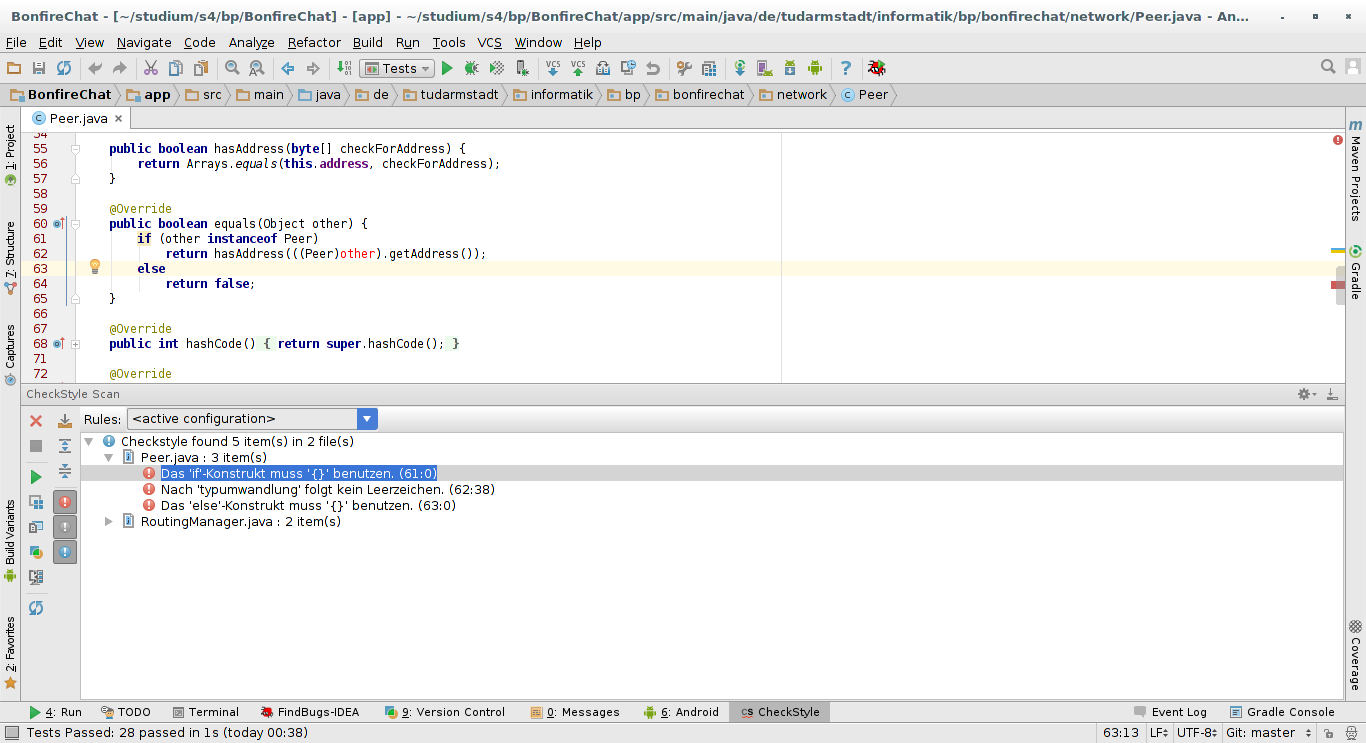
\includegraphics[width=17.5cm]{belege/checkstyle/checkstyle-idea-screenshot.png}
